%% LyX 2.0.5.1 created this file.  For more info, see http://www.lyx.org/.
%% Do not edit unless you really know what you are doing.
\documentclass{article}
\usepackage[sc]{mathpazo}
\usepackage{geometry}
\geometry{verbose,tmargin=2.5cm,bmargin=2.5cm,lmargin=2.5cm,rmargin=2.5cm}
\setcounter{secnumdepth}{2}
\setcounter{tocdepth}{2}
\usepackage{url}
\usepackage[unicode=true,pdfusetitle,
 bookmarks=true,bookmarksnumbered=true,bookmarksopen=true,bookmarksopenlevel=2,
 breaklinks=false,pdfborder={0 0 1},backref=false,colorlinks=false]
 {hyperref}
\hypersetup{
 pdfstartview={XYZ null null 1}}
\usepackage{breakurl}
\usepackage{Sweave}
\begin{document}
\Sconcordance{concordance:report.tex:report.Rnw:%
1 16 1 1 0 2 1 1 3 2 0 1 1 3 0 1 2 10 1 2 2 3 1 1 7 5 1}


\begin{Schunk}
\begin{Sinput}
> # set global chunk options
> opts_chunk$set(fig.path='figure/minimal-', fig.align='center', fig.show='hold')
> options(replace.assign=TRUE,width=90)
\end{Sinput}
\end{Schunk}


\title{A Summary of Time Series Analysis Result}


\author{Carol Zhang}

\maketitle
This is the report generated automatically from \textbf{R} with package \textbf{knitr}. 
Here are some simple visualizing plots of the data:

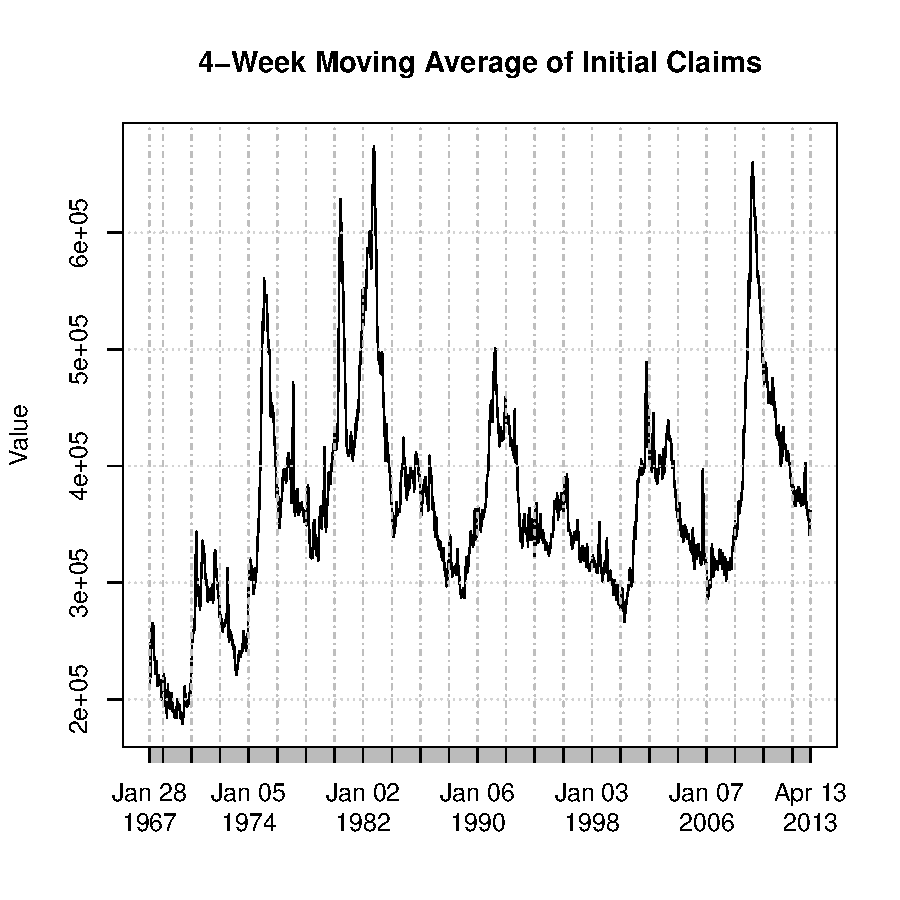
\includegraphics{report-boring-random}

The first element of \texttt{x} is 0.144958306409317. Boring boxplots
and histograms recorded by the PDF device:


Do the above chunks work? You should be able to compile the \TeX{}
document and get a PDF file like this one: \url{https://bitbucket.org/stat/knitr/downloads/knitr-minimal.pdf}.
The Rnw source of this document is at \url{https://github.com/yihui/knitr/blob/master/inst/examples/knitr-minimal.Rnw}.

\end{document}
